\subsection{Zählrohr-Charakteristik}
Die Zählrohr-Charakteristik ist in Abbildung \ref{picA}, welche 
die Messdaten aus Tabelle \ref{taba1} verwendet, abgebildet. 
\begin{table}[h!]
	\begin{center}
		\begin{tabular}{cc}
			Anodenspannung [V] & Anodenstrom [mA]\\ \hline
			10	&0,044\\
			20	&0,088\\
			30	&0,108\\
			40	&0,119\\
			50	&0,126\\
			60	&0,128\\
			70	&0,132\\
			80	&0,135\\
			90	&0,138\\
			100	&0,141\\
			110	&0,144\\
			120	&0,146\\
			130	&0,147\\
			140	&0,149\\
			150	&0,150\\
			160	&0,151\\
			170	&0,152\\
			180	&0,154\\
			190	&0,155\\
			200	&0,156\\
			210	&0,157
		\end{tabular}
		\caption{Kennlinie 1 (Heizwerte: 4,2V; 2,1A)}
		\label{taba1}
	\end{center}
\end{table} 	\begin{figure}[h]
		\begin{center}
		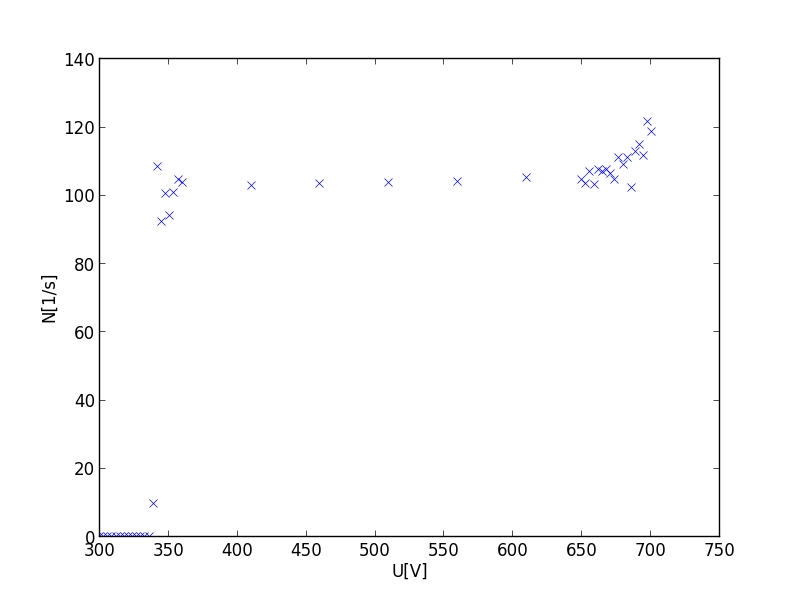
\includegraphics[scale=0.75]{picA.jpg}
		\caption{Grafisches Auftragen der Messwerte zur Zählrohr-Charakteristik}
		\label{picA}
		\end{center}	
	\end{figure}
\FloatBarrier
Die Länge des Plateau-Bereiches lässt sich darauf aufbauend auf ungefähr
290 Volt, von 360 Volt bis 650 Volt, abschätzen. Dieser Bereich ist in 
Abbildung \ref{picAlinregwitherrors} mit einem Messfehler von unter $1\%$ (\cite{anleitung}, Seite 226) 
noch einmal dargestellt, wobei in diesem Bereich (vgl. \ref{taba1})eine lineare 
Ausgleichsrechnung \cite{linreg} (Gl. \ref{eqlinrega}) programmiert in Python durchgeführt wurde:
\begin{align}
y&=a*x+b \\
\Leftrightarrow N&=0,0050\frac{1}{\text{s V}}*U+101,4606\frac{1}{\text{s}} \label{eqlinrega} \\
a&=0,0050\frac{1}{\text{s V}} \label{eqalinrega}\\
\Delta a&=38,0\% \\
b&=101,4606\frac{1}{\text{s}}\\
\Delta b&=0,9\%
\end{align}
	\begin{figure}[h]
		\begin{center}
		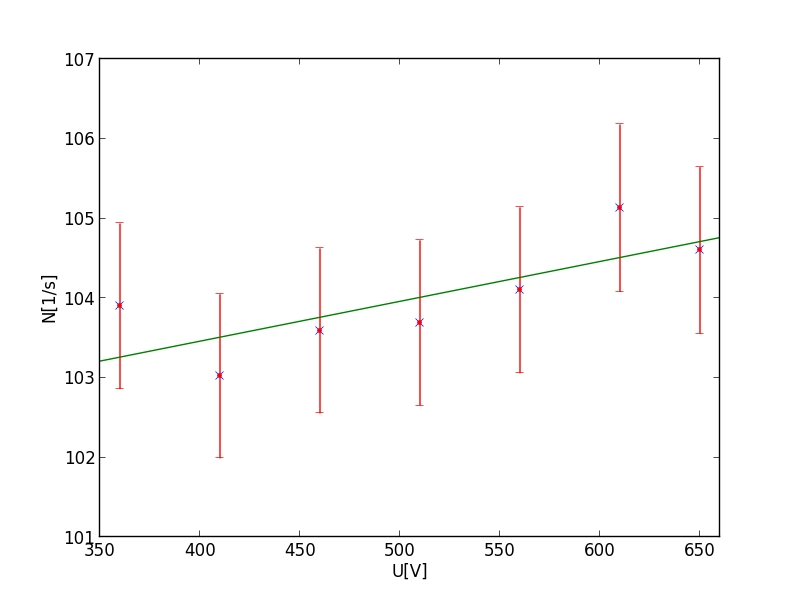
\includegraphics[scale=0.75]{picAlinregwitherrors.jpg}
		\caption{Plateau-Bereich der Zählrohr-Charakteristik}
		\label{picAlinregwitherrors}
		\end{center}	
	\end{figure}
\FloatBarrier
Aus der Linearen Regression lässt sich dann die Plateau-Steigung von $0,5\% \text{ pro } 
100 \text{ Volt }$(Gl. \ref{eqalinrega}) ablesen.
\subsection{Totzeitbestimmung nach der Zwei-Quellen-Methode}
\FloatBarrier
\begin{table}[h]
	\begin{center}
		\begin{tabular}{ccc}
			$N_1$[1/s]&$N_2$[1/s]&$N_{1+2}$[1/s] \\ \hline
			234,26&12,74&245,60\\
		\end{tabular}
		\caption{Zwei-Quellen-Methode}
		\label{tabc2}
	\end{center}
\end{table}
Die Totzeit lässt sich nach Gleichung \ref{2} aus der Zwei-Quellen-Methode mit Tabelle \ref{tabc2} berechnen,
der Fehler ergibt sich aus Gleichung \ref{totzeit2fehler}.
\begin{align}
\frac{N_{1+2}}{1 - T N_{1+2}}&=\frac{N_1}{1 - T N_1} + \frac{N_2}{1 - T N_2} \label{totzeit2fehler}\\
T= 234,5 \mu\text{s} \label{eqtot2}\\
\Delta T&=0,017\%
\end{align}
\subsection{Pro Teilchen freigesetzte Ladungsmenge im Zählrohr}
\FloatBarrier
Die pro Teilchen freigesetzte Ladungsmenge im Zählrohr lässt sich nach Gleichung \ref{ladungsmenge}
berechnen.
Daraus ergeben sich die Ladungsmengen in Tabelle \ref{tabd1} beziehungsweise Abbildung \ref{picD}.
In dem linearen Bereich, abgeschätzt von U$=360$V bis U$=650$V,wurde eine lineare Ausgleichsrechnung \cite{linreg} (Gl. \ref{eqlinregd}) 
programmiert in Python durchgeführt:
\begin{align}
y&=a*x+b \\
\Leftrightarrow Q/e&=(1,2093 * 10^8) \frac{1}{\text{V}} *U+ (-3,1548 * 10^10) \label{eqlinregd} \\
a&=(1,2093 * 10^8) \frac{1}{\text{V}} \label{eqalinregd}\\
\Delta a&=1,3\% \\
b&=-3,1548 * 10^10\\
\Delta b&=2,8\%
\end{align}
\begin{table}[h]
	\begin{center}
		\begin{tabular}{cc}
			U[V]&$\Delta Q [\frac{\text{C}}{e}] * 10^9$ \\ \hline
			339&63,68\\
			342&11,50\\
			345&13,53\\
			348&12,40\\
			351&13,25\\
			354&12,39\\
			357&11,92\\
			360&12,01\\
			410&18,17\\
			460&24,10\\
			510&30,09\\
			560&35,97\\
			610&41,55\\
			650&47,73\\
			653&48,29\\
			656&46,66\\
			659&48,33\\
			662&46,36\\
			665&52,44\\
			668&52,20\\
			671&52,79\\
			674&53,75\\
			677&50,56\\
			680&51,58\\
			683&50,60\\
			686&54,91\\
			689&49,79\\
			692&48,88\\
			695&50,28\\
			698&46,15\\
			701&52,62
		\end{tabular}
		\caption{freigesetzte Ladungsmenge im Zählrohr}
		\label{tabd1}
	\end{center}
\end{table} 	\begin{figure}[h]
		\begin{center}
		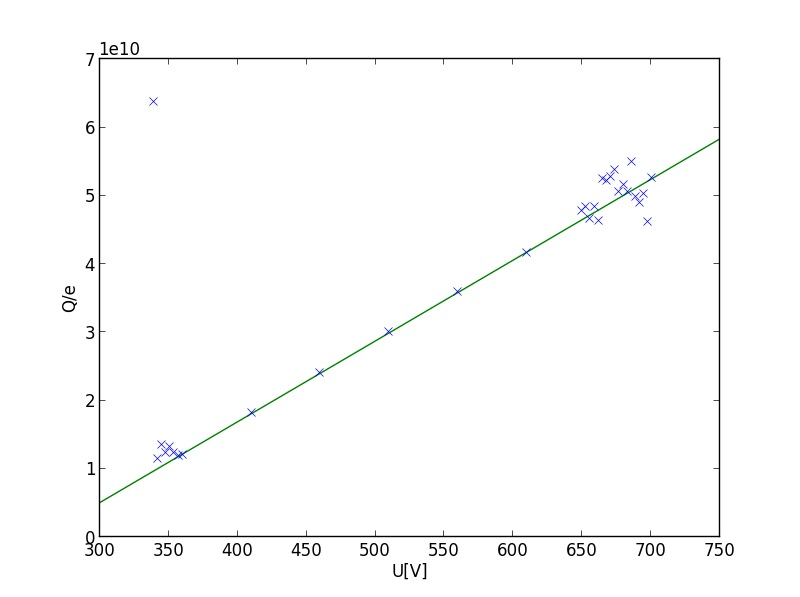
\includegraphics[scale=0.75]{picD.jpg}
		\caption{freigesetzte Ladungsmenge im Zählrohr}
		\label{picD}
		\end{center}	
	\end{figure}
\FloatBarrier